\documentclass{article}
\usepackage[utf8]{inputenc}
\usepackage{fancyhdr}
\usepackage{parskip}
\usepackage{multicol}
\usepackage[a4paper, total={6in, 8in}]{geometry}
\usepackage{graphicx}
\usepackage[toc,page]{appendix}

\title{COMP2208 - Search Methods Coursework}
\author{Daniel Best (Student ID: 29777127)}

\pagestyle{fancy}
\fancyhf{}
\renewcommand{\headrulewidth}{0pt}
\renewcommand{\footrulewidth}{0.5pt}
\lfoot{Daniel Best}
\cfoot{\thepage}
\rfoot{COMP2208}
\graphicspath{ {./images/} }

\begin{document}
	\maketitle
	
	\newpage
	
	\section{Approach}
	My approach to this assignment was to first create support classes that would handle any details that didn't directly relate to the search algorithm itself. These are as follows:
	
	\subsection{Node}
	This class defines both a singular node in the tree structure, as well as the entire tree structure itself by means of its \textbf{parent} and \textbf{children} variables. It contains a single \textbf{Grid} object, the \textbf{value} variable. It also implements the Comparable interface, where it compares an optional \textbf{estimatedCost} variable - a feature that was specifically added for the A* Search algorithm.

	\subsection{Grid}
	A class that handles the state by means of manipulating a \textbf{char[][]} multidimensional array. This class stores the actual state of the problem, storing the location of the \textbf{agent} ($\neg$) and all of the non-white space blocks; it also allows for that state to be manipulated in a multitude of ways:
	
	\begin{itemize}
		\item Generates the start and solution state.
		\item Moves the agent in the grid, thereby changing the location of both the agent and the block it moves to.
		\item Calculates the \textbf{Manhattan distance} between the Grid and another Grid object passed to it, which is used as the heuristic for A* Search.
	\end{itemize}
	
	\subsection{Search}
	An abstract class that defines a common start and solution state for each of the individual search methods, and provides a common \textbf{expandNode()} method, which generates the children of a given node.
	
	Using this \textbf{Search} class, I was able to easily implement a class for each of the four search algorithms:
	
	\subsection{Breadth First Search (BFS)}
	Uses a \textbf{Queue} to store expanded nodes, meaning nodes are checked in the order they are expanded.
	
	\subsection{Depth First Search (DFS)}
	Uses a \textbf{Stack} to store expanded nodes, meaning the last node to expanded is checked next.
	
	\subsection{Iterative Deepening Search (IDS)}
	Uses \textbf{Depth Limited Search (DLS)}, a modified version of \textbf{DFS} that does not expand nodes at a given \textbf{depth}, which then iteratively increases this limit. 
	
	\subsection{A* Heuristic Search}
	Makes use of an evaluation function to determine which node to pick next, which is the \textbf{depth} of the node plus the \textbf{Manhattan distance (heuristic)} to the solution.
	
	\section{Evidence of Search Methods}
	When testing my search methods, I found 21 start states that each corresponded to a problem which has an optimal solution at a different depth (from 0 to 20). The solution state was always the same, as specified by the problem in the assignment briefing.
	
	\subsection{Breadth First Search (BFS)}
	\textbf{Example 1 (depth 4):}
	
	In this initial state, the agent has three possible directions that it can move.
	\begin{figure}[h]
		\centering
		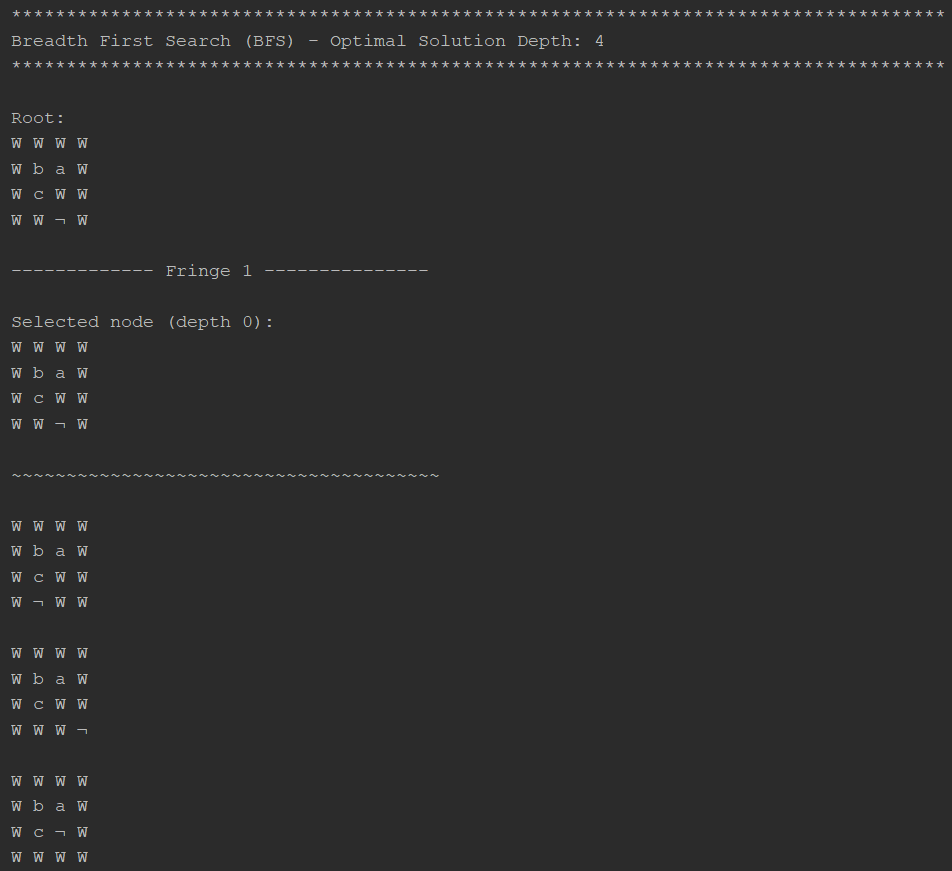
\includegraphics[height=0.75\textheight]{BFS-1-1.png}
	\end{figure}

	These three new nodes are then expanded in the order that they were first generated.
	\begin{multicols}{3}[\columnsep=2cm]
		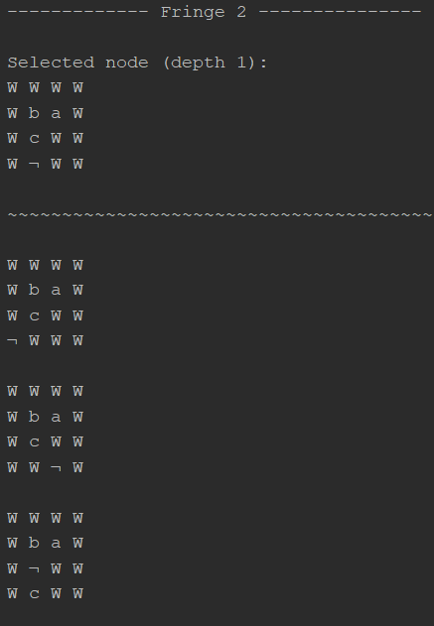
\includegraphics[width=0.3\textwidth,keepaspectratio]{BFS-1-2-1.png}
		\columnbreak
		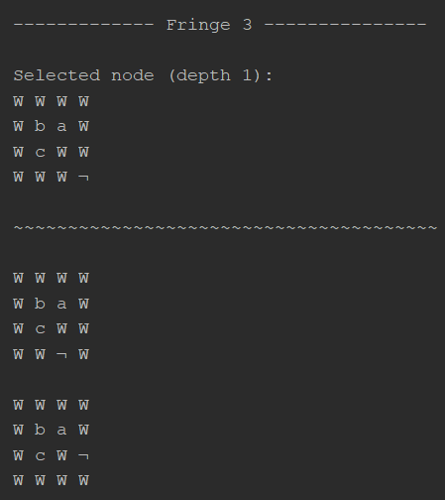
\includegraphics[width=0.3\textwidth,keepaspectratio]{BFS-1-2-2.png}
		\columnbreak
		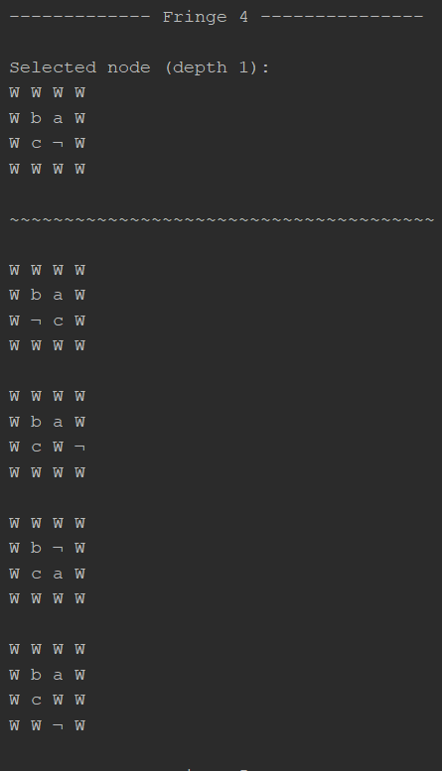
\includegraphics[width=0.3\textwidth,keepaspectratio]{BFS-1-2-3.png}
	\end{multicols}

	The algorithm then expands the first child node in \textbf{Fringe 2}, which generates the first nodes that are at a depth of 2.
	\begin{figure}[h]
		\centering
		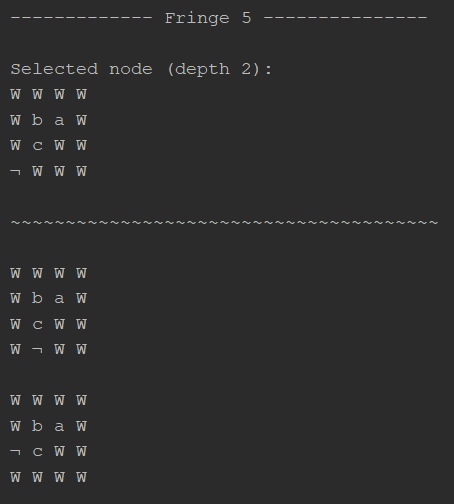
\includegraphics{BFS-1-3.png}
	\end{figure}

	This process then repeats indefinitely until the correct node is found. At the 21st expansion to the fringe, we can see the correct node being found.
	\begin{figure}[h]
		\centering
		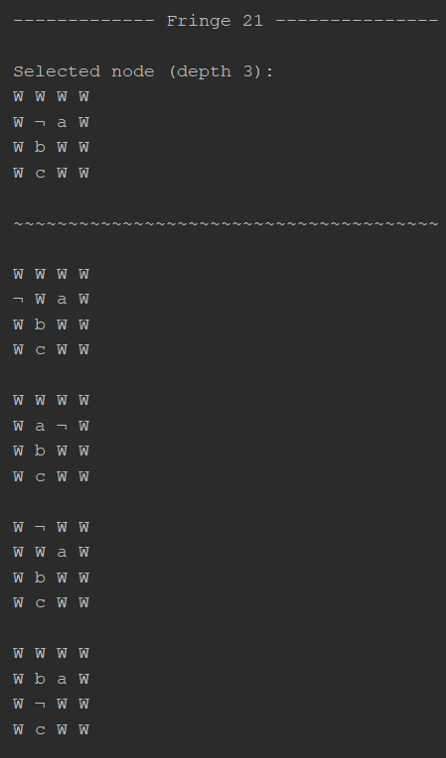
\includegraphics{BFS-1-4.png}
	\end{figure}

	However, due to the uninformed nature of the algorithm, it does not recognise this as it only checks if it is in the goal state when taking it off the \textbf{Queue}. It therefore continues to go through each node on depth 3, and all the nodes in depth 4 that exist prior to that node - a further 44 expansions. 
	
	\newpage
	\textbf{Fringe 65} shows the node that was generated prior to the goal state node being expanded.
	
	\begin{figure}[h]
		\centering
		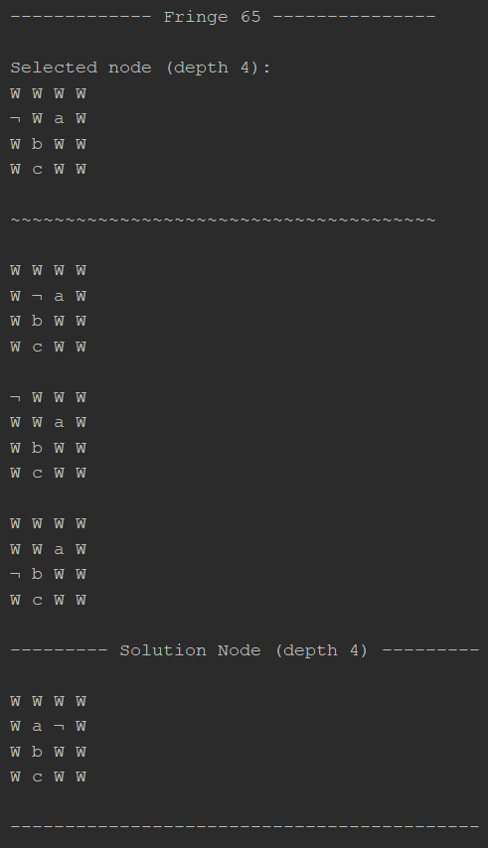
\includegraphics[height=0.4\textheight]{BFS-1-5.png}
	\end{figure}
	
	The following is a breakdown of the solution of this problem, as retrieved by this search.
	
	\begin{figure}[h]
		\centering
		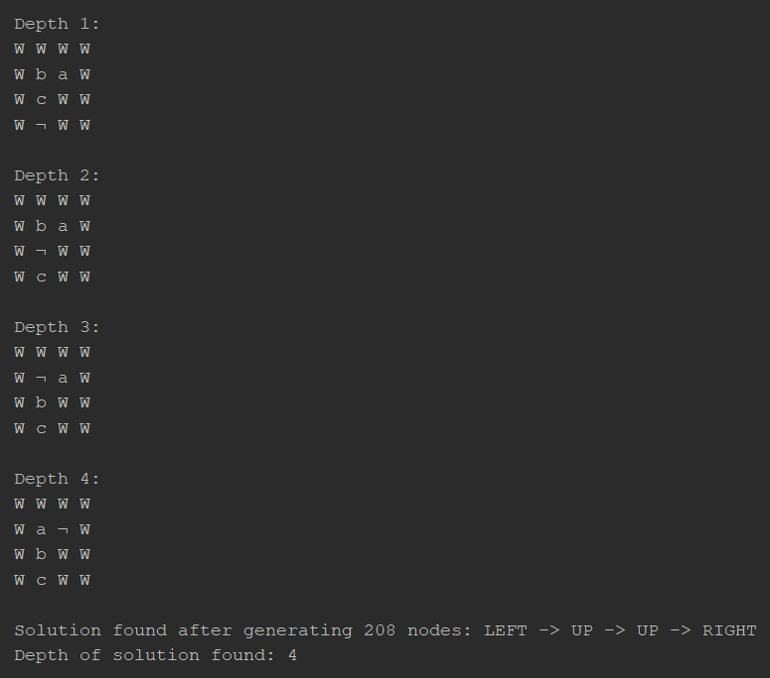
\includegraphics[height=0.33\textheight]{BFS-1-6.png}
	\end{figure}
	
	\newpage
	\textbf{Example 2 (depth 14):}
	
	The original problem provided for the assignment has an optimal solution at \textbf{depth 14}, but running BFS on it causes a \textbf{Java Heap space error} due to the number of generated nodes (space complexity).
	
	The algorithm starts in the same way that it did for the previous problem, by expanding the root node, and then by expanding each subsequent child in the order that they were generated.
	
	\begin{figure}[h]	
		\centering
		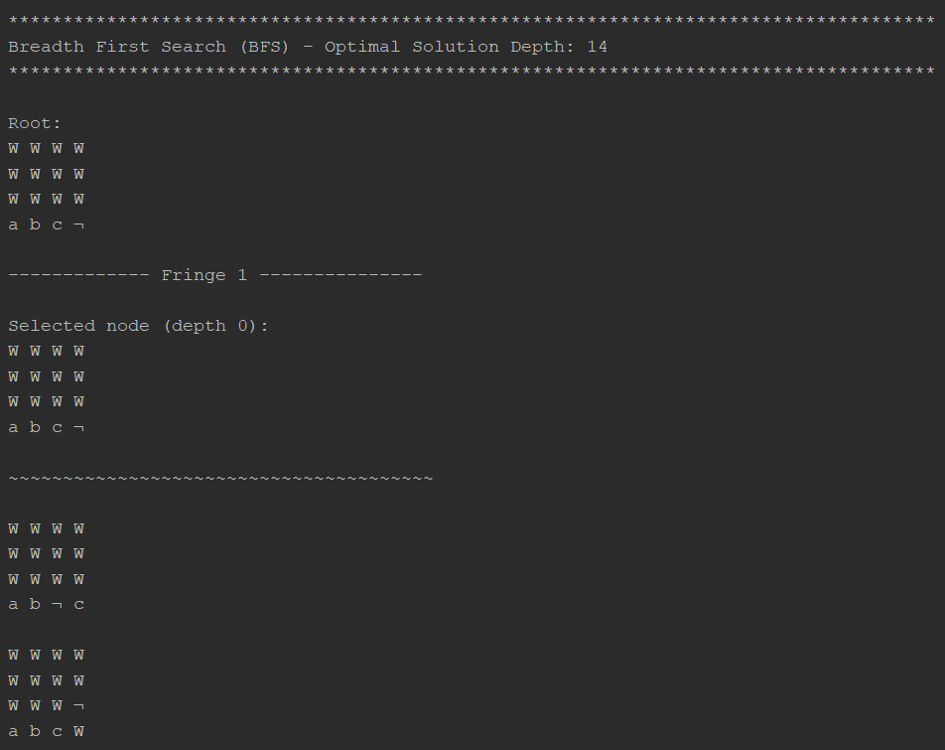
\includegraphics[width=\textwidth,keepaspectratio]{BFS-2-1.png}
	\end{figure}

	\newpage
		
	\begin{multicols}{2}[\columnsep=2cm]
		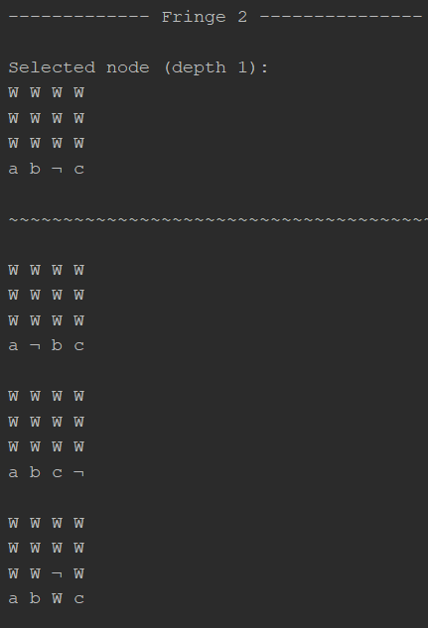
\includegraphics[width=0.4\textwidth,keepaspectratio]{BFS-2-2-1.png}
		\columnbreak
		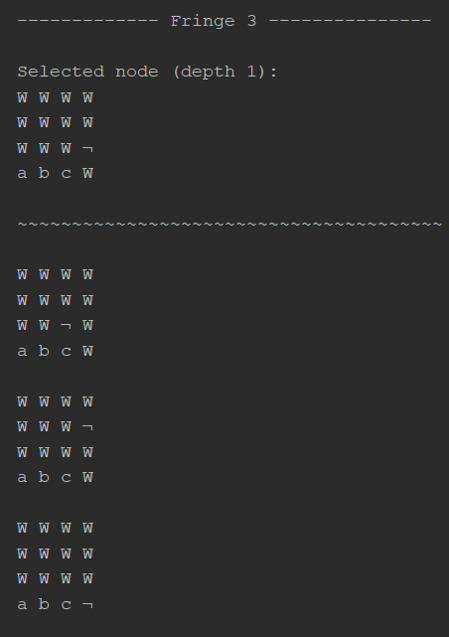
\includegraphics[width=0.4\textwidth,keepaspectratio]{BFS-2-2-2.png}
	\end{multicols}
	
	It then continues this process of first checking all of the nodes on a depth in the order they were generated, and then moving down to the next depth.
	
	Eventually however, it will run into an \textbf{OutOfMemoryException} due to running out of Java Heap space.
	
	\begin{figure}[h]	
		\centering
		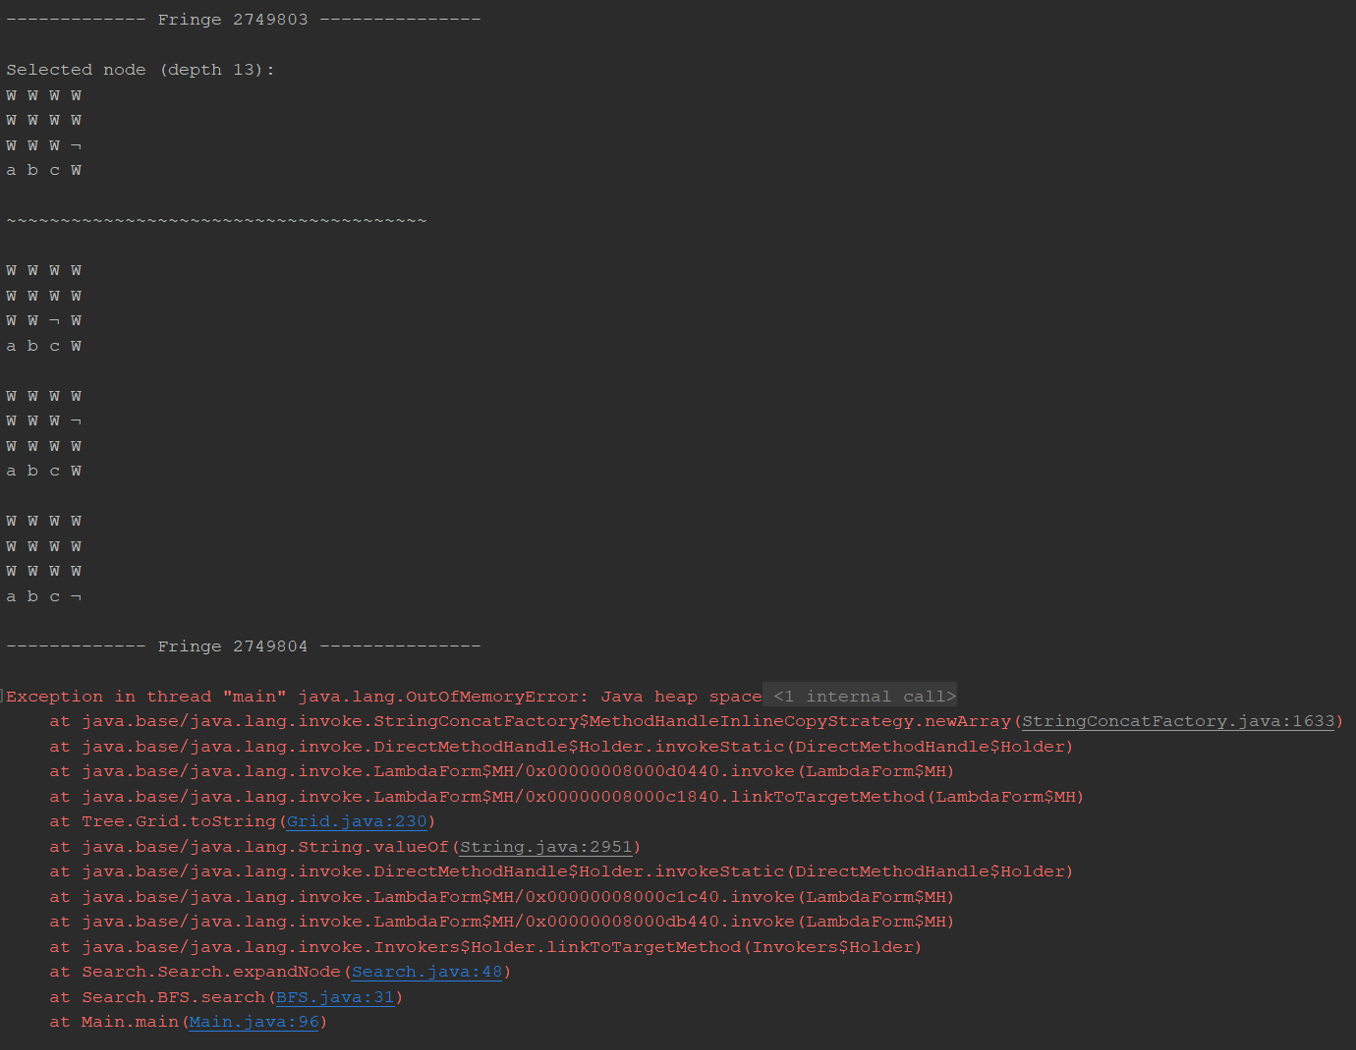
\includegraphics[height=0.4\textheight,keepaspectratio]{BFS-2-3.png}
	\end{figure}
	
	\newpage
	\subsection{Depth First Search (DFS)}
	\textbf{Example 1 (depth 5):}
	
	Implementing DFS for this type of problem has an obvious flaw in that the nodes are generated in an ordered manner. In the case of my algorithm, this is left, right, up and down. As such, the node added to the top of the \textbf{Stack} will always be the last possible direction. In this particular example, the agent will keep moving down and then back up again, since these will be the latest nodes generated.
	
	\begin{multicols}{2}[\columnsep=2cm]
		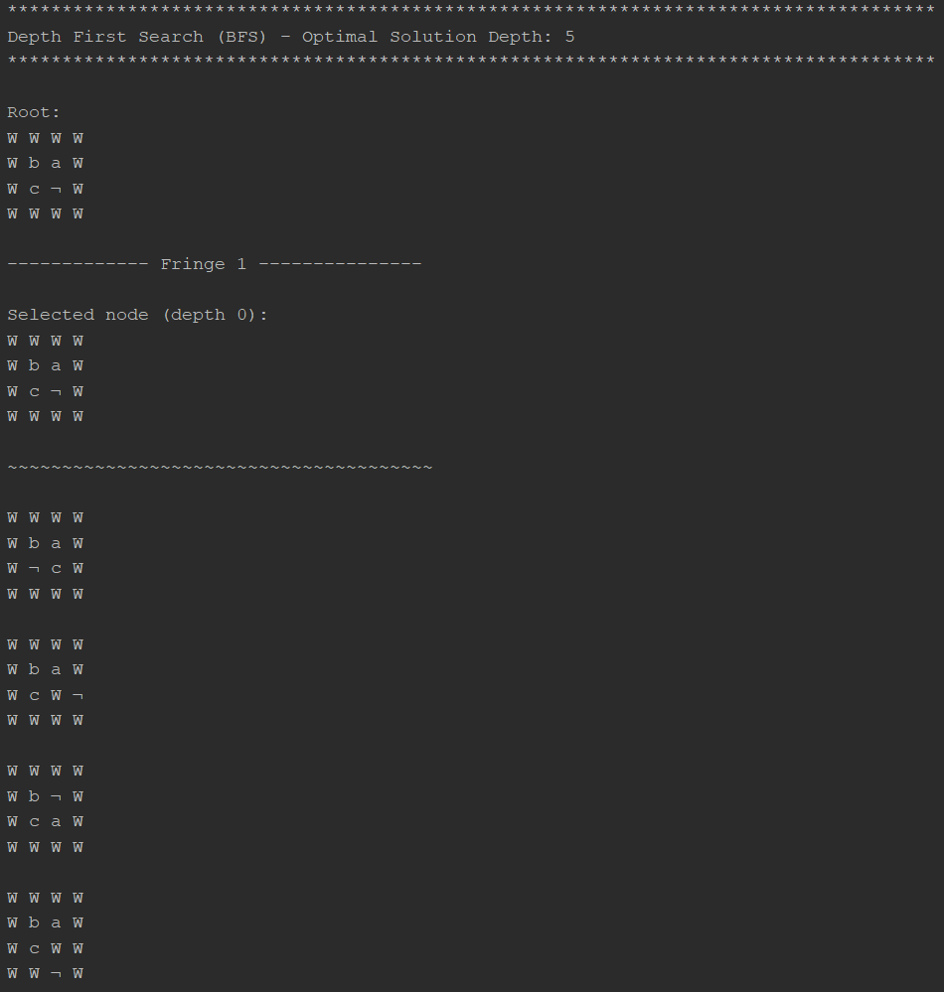
\includegraphics[width=0.5\textwidth,keepaspectratio]{DFS-1-1.png}
		\columnbreak
		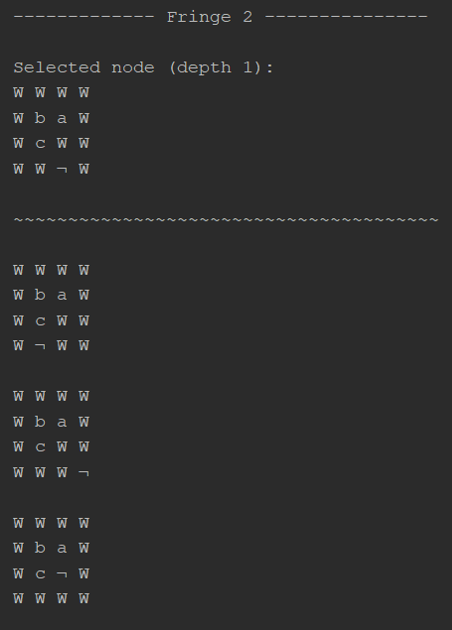
\includegraphics[width=0.4\textwidth,keepaspectratio]{DFS-1-2.png}
	\end{multicols}
	
	\newpage
	This means that unless modified accordingly, i.e. so the order of the generated nodes is randomised, the algorithm will almost certainly never find a solution.
		
	\begin{multicols}{2}[\columnsep=2cm]
		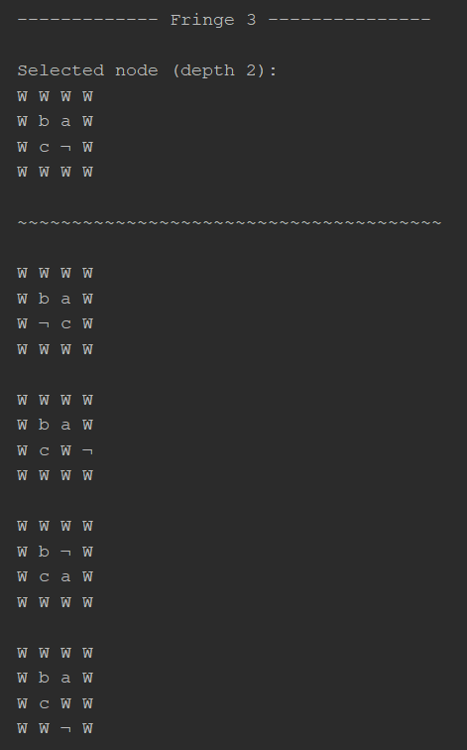
\includegraphics[width=0.4\textwidth,keepaspectratio]{DFS-1-3.png}
		\columnbreak
		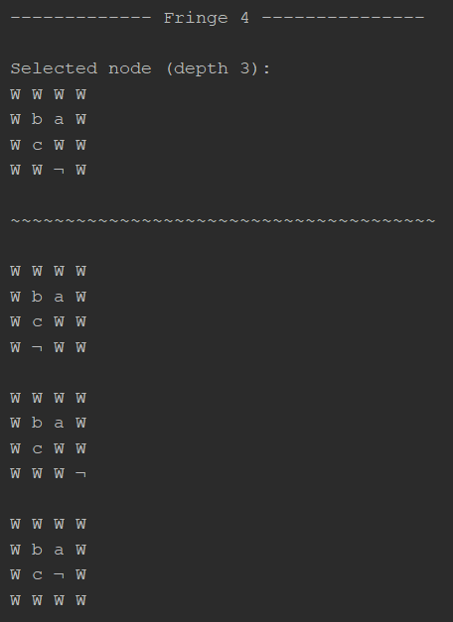
\includegraphics[width=0.4\textwidth,keepaspectratio]{DFS-1-4.png}
	\end{multicols}

	\newpage
	Eventually, this will cause an \textbf{OutOfMemoryException}, since it will repeat this process indefinitely, with the only difference being that the depth has increased by one each time.
	
	\begin{multicols}{2}[\columnsep=2cm]
		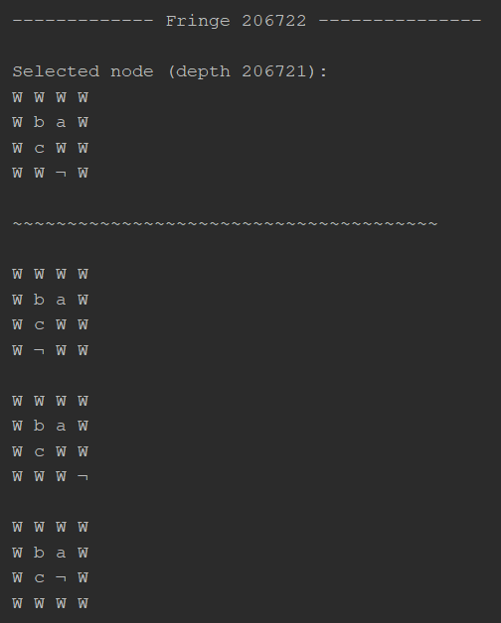
\includegraphics[width=0.4\textwidth,keepaspectratio]{DFS-1-5.png}
		\columnbreak
		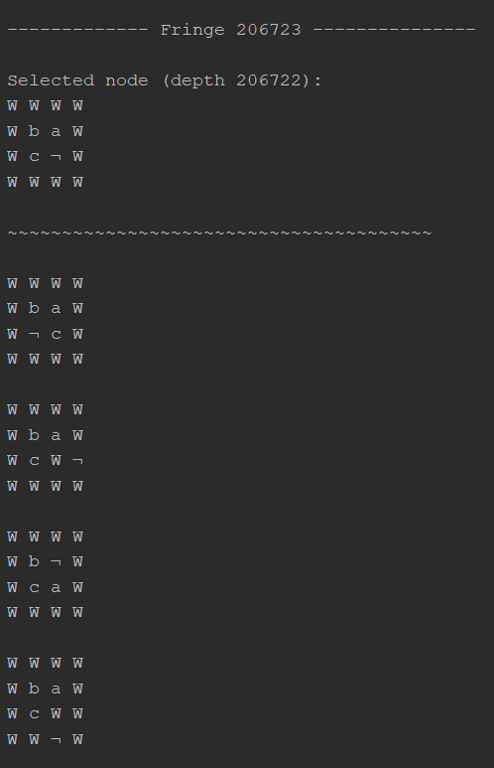
\includegraphics[width=0.4\textwidth,keepaspectratio]{DFS-1-6.png}
	\end{multicols}

	\newpage
	\textbf{Example 2 (depth 5 with random order):}
	
	In order to get DFS working with this problem, the order in which the generated nodes are placed onto the \textbf{Stack} should be randomised. This is done by using the \textbf{Collections.shuffle()} function on the children list. Below, we can see the effect this has on the third and fourth node expansion.
	
	\begin{multicols}{2}[\columnsep=2cm]
		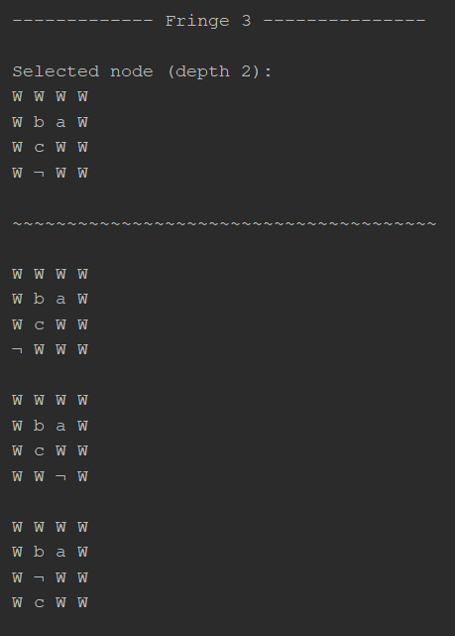
\includegraphics[width=0.4\textwidth,keepaspectratio]{DFS-2-1.png}
		\columnbreak
		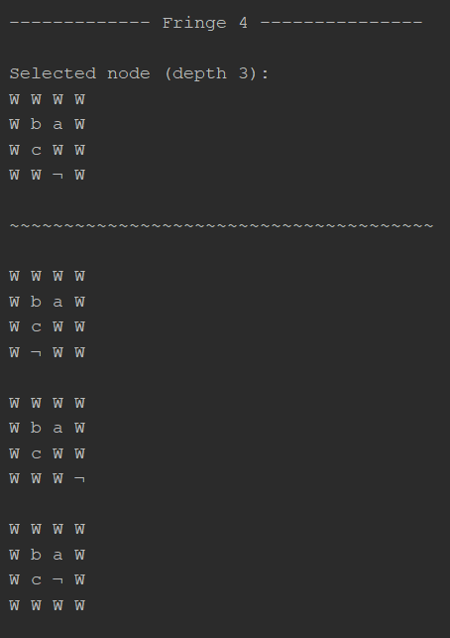
\includegraphics[width=0.4\textwidth,keepaspectratio]{DFS-2-2.png}
	\end{multicols}

	\newpage
	By completely arbitrary movements, the algorithm will eventually find some solution.
	
	\begin{figure}[h]	
		\centering
		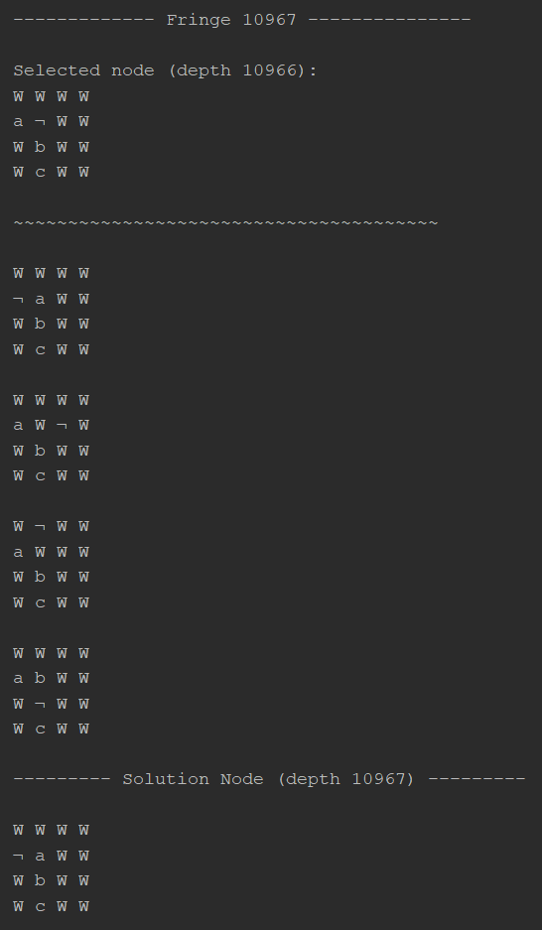
\includegraphics[height=0.7\textheight,keepaspectratio]{DFS-2-3.png}
	\end{figure}

	However, this solution is almost guaranteed to not be the optimal solution. The solution returned here is in 10967 steps, whereas the optimal solution for this problem is in merely 5.
	
	\begin{figure}[h]	
		\centering
		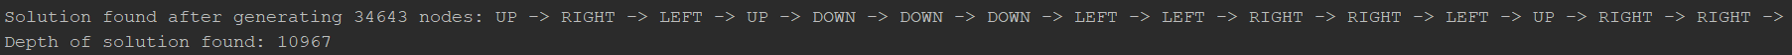
\includegraphics[width=\textwidth,keepaspectratio]{DFS-2-4.png}
	\end{figure}

	\newpage
	Due to the random nature of this algorithm, the solution returned is very likely to be different each time, with the below showing what the algorithm returns on another run-through.
	
	\begin{figure}[h]	
		\centering
		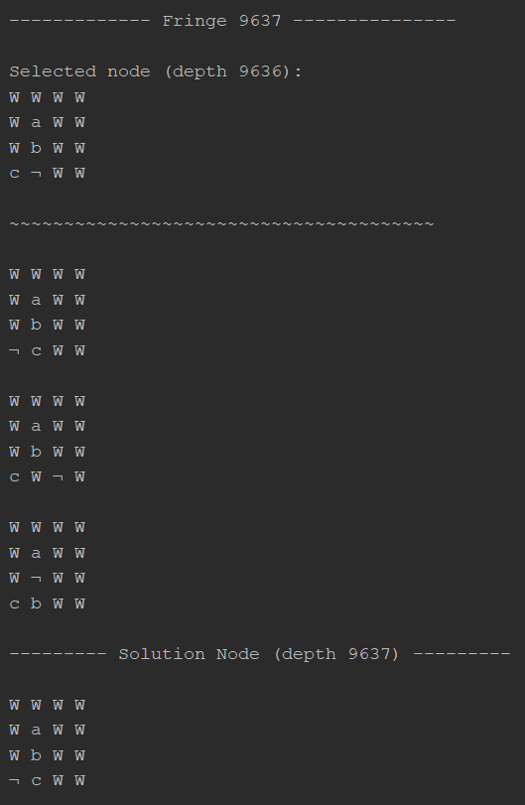
\includegraphics[height=0.6\textheight,keepaspectratio]{DFS-2-5.png}
	\end{figure}
	
	\newpage
	\subsection{Iterative Deepening Search (IDS)}
	\textbf{Example 1 (depth 6):}
	
	The IDS algorithm begins by calling DLS with a limit of depth 1. The agent in this initial state has three possible directions that it can move in. Each of these children are then also checked to see if they are the goal state.
	
	\begin{figure}[h]
		\centering
		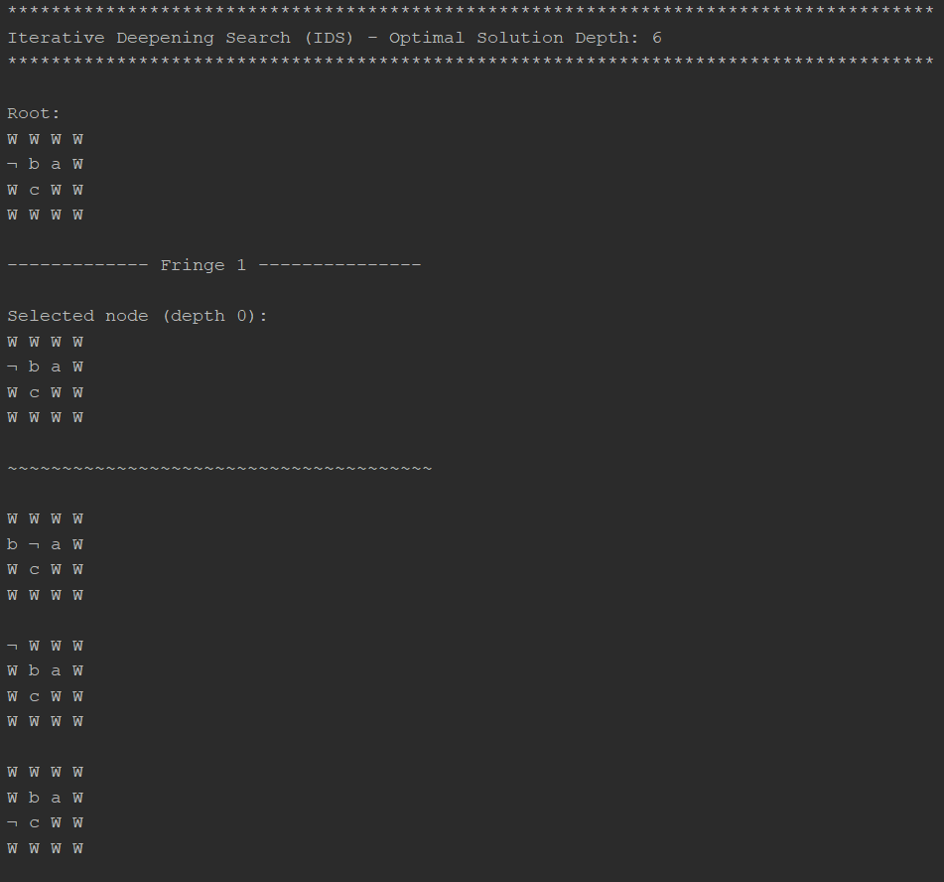
\includegraphics[height=0.7\textheight]{IDS-1-1.png}
	\end{figure}

	\newpage
	The IDS then increases the limit to 2, and performs another DLS on this limit.
	
	\begin{figure}[h]
		\centering
		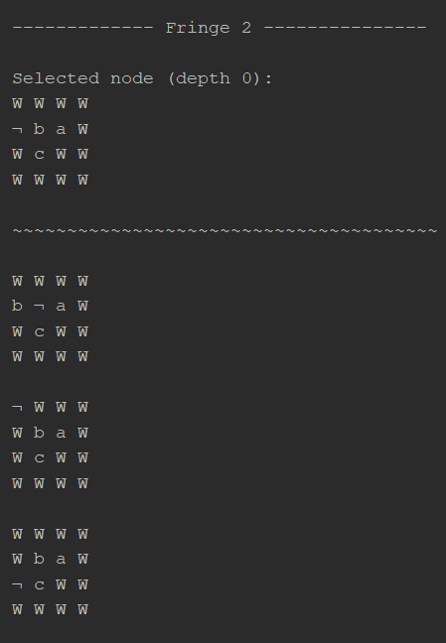
\includegraphics[height=0.7\textheight]{IDS-1-2.png}
	\end{figure}

	\newpage
	However, because the limit is now 2, we also expand the nodes at depth 1, and then check the nodes at depth 2 that are generated from these expansions.
	\begin{multicols}{3}[\columnsep=2cm]
		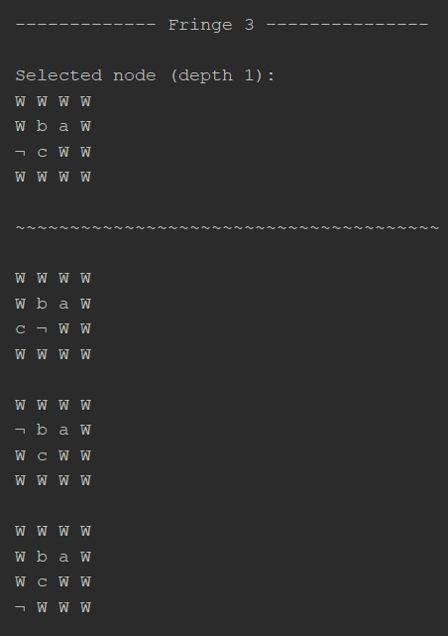
\includegraphics[width=0.3\textwidth,keepaspectratio]{IDS-1-3-1.png}
		\columnbreak
		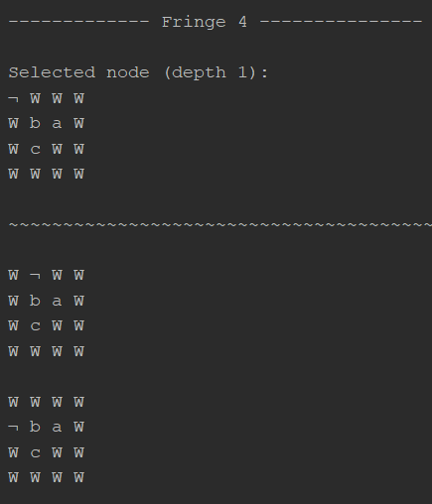
\includegraphics[width=0.3\textwidth,keepaspectratio]{IDS-1-3-2.png}
		\columnbreak
		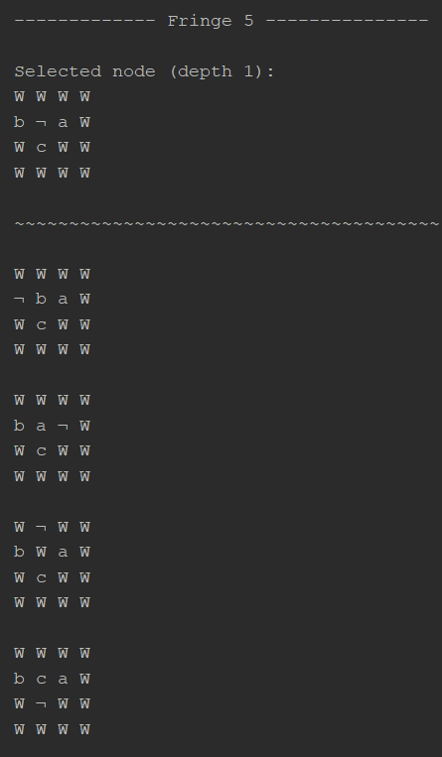
\includegraphics[width=0.3\textwidth,keepaspectratio]{IDS-1-3-3.png}
	\end{multicols}

	\newpage
	Since none of these nodes contain the goal state (which can actually be found at depth 6), we repeat this process until the goal state is found.
	
	\begin{figure}[h]
		\centering
		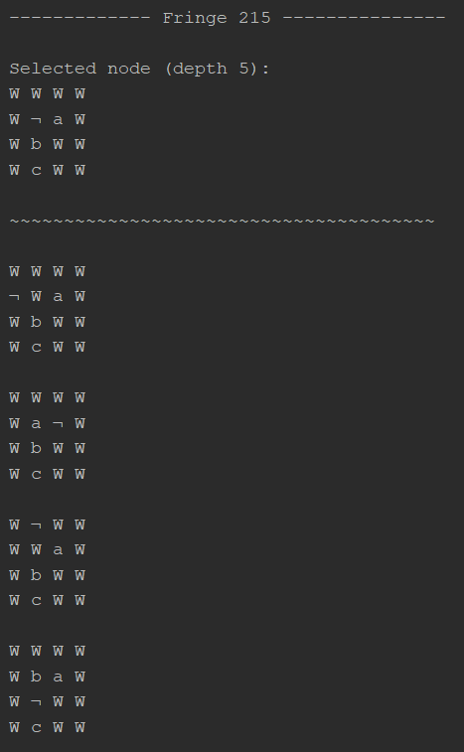
\includegraphics[height=0.7\textheight]{IDS-1-4.png}
	\end{figure}

	\newpage
	If we look at the node expansions prior to this, we can see the DFS nature of the algorithm, as the next node selected is always the last generated. The next node expansion contains the goal state that was seen in the previous image (labelled \textbf{Fringe 215}).
	\begin{multicols}{3}[\columnsep=2cm]
		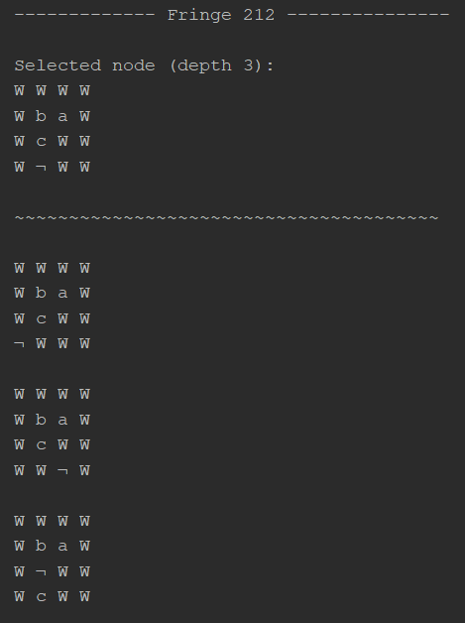
\includegraphics[width=0.3\textwidth,keepaspectratio]{IDS-1-5-1.png}
		\columnbreak
		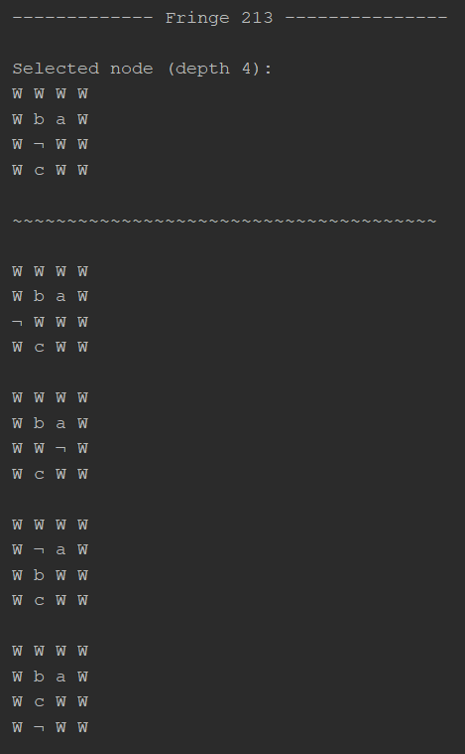
\includegraphics[width=0.3\textwidth,keepaspectratio]{IDS-1-5-2.png}
		\columnbreak
		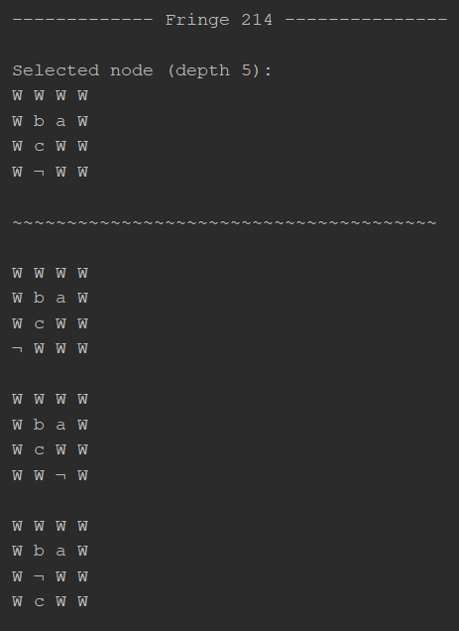
\includegraphics[width=0.3\textwidth,keepaspectratio]{IDS-1-5-3.png}
	\end{multicols}
	
	\newpage
	The optimal solution was therefore found at depth 6.
	
	\begin{figure}[h]
		\centering
		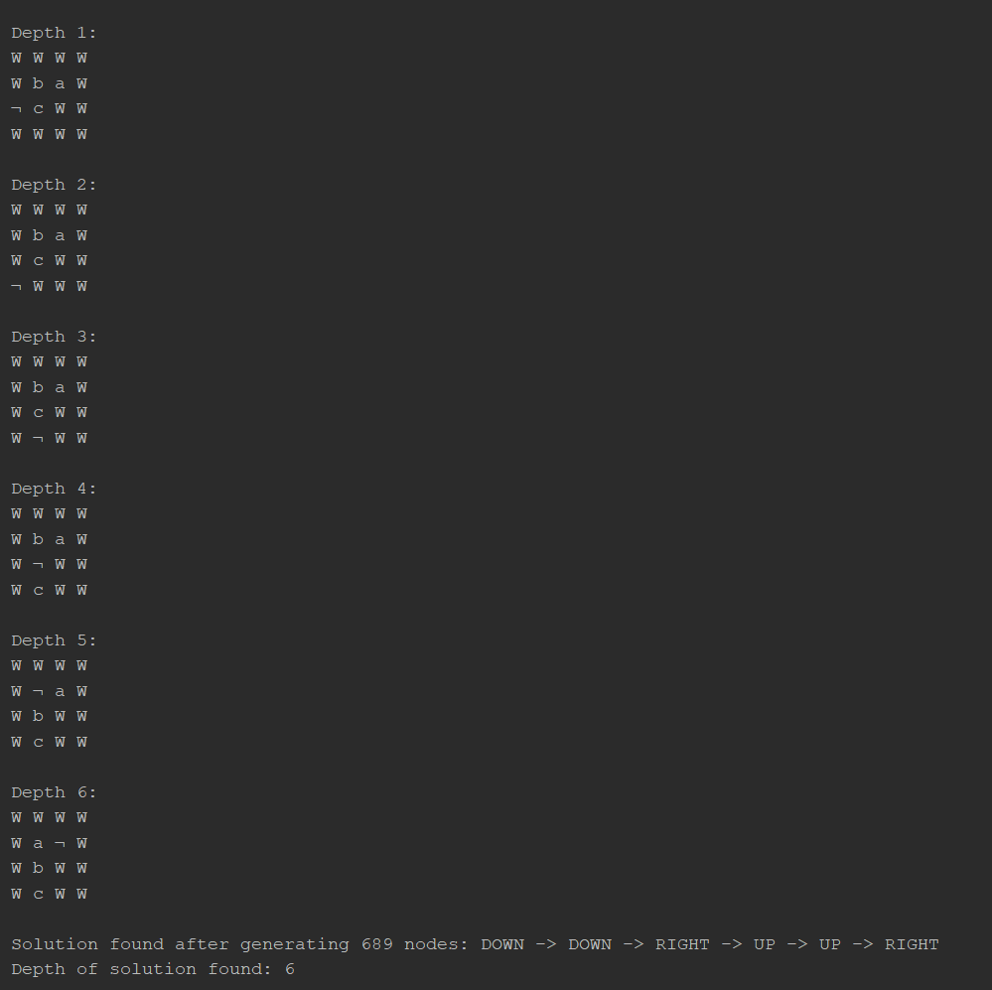
\includegraphics[height=0.6\textheight]{IDS-1-6.png}
	\end{figure}

	\newpage
	\textbf{Example 2 (depth 15):}
	
	Whilst IDS has a better space complexity than BFS because it handles works in a DFS manner with its node expansion, it is not immune to space constraints at a large enough problem size. The following problem has an optimal solution at a depth of 15.
	
	\begin{figure}[h]
		\centering
		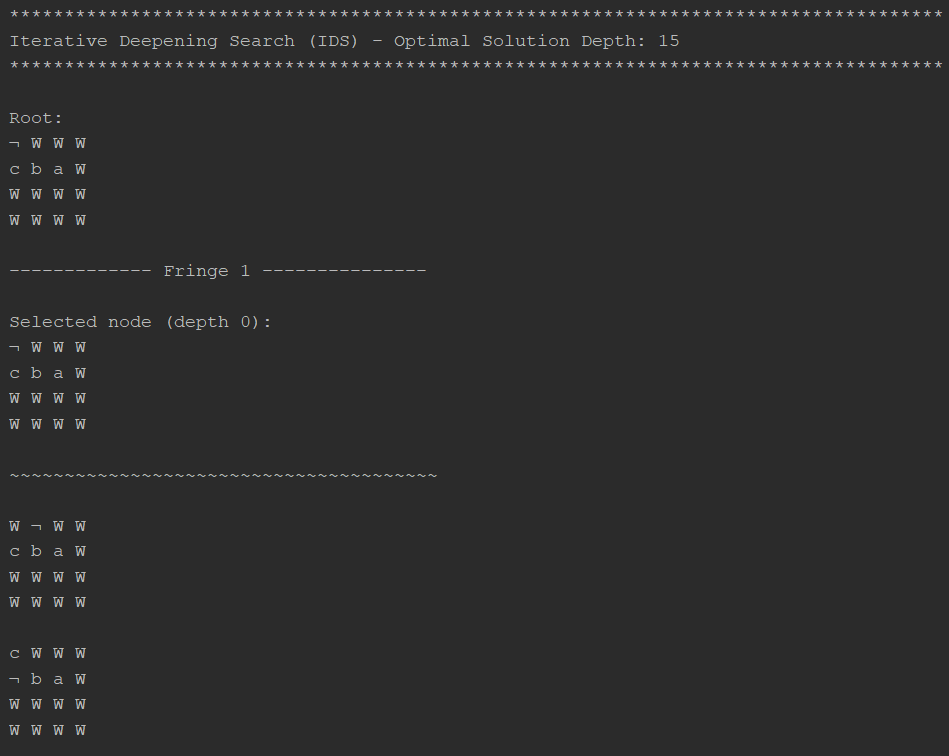
\includegraphics[height=0.6\textheight]{IDS-2-1.png}
	\end{figure}
	
	\newpage
	This means that like BFS, a failed IDS at a certain depth will cause a \textbf{Java heap space error}.
	
	\begin{figure}[h]
		\centering
		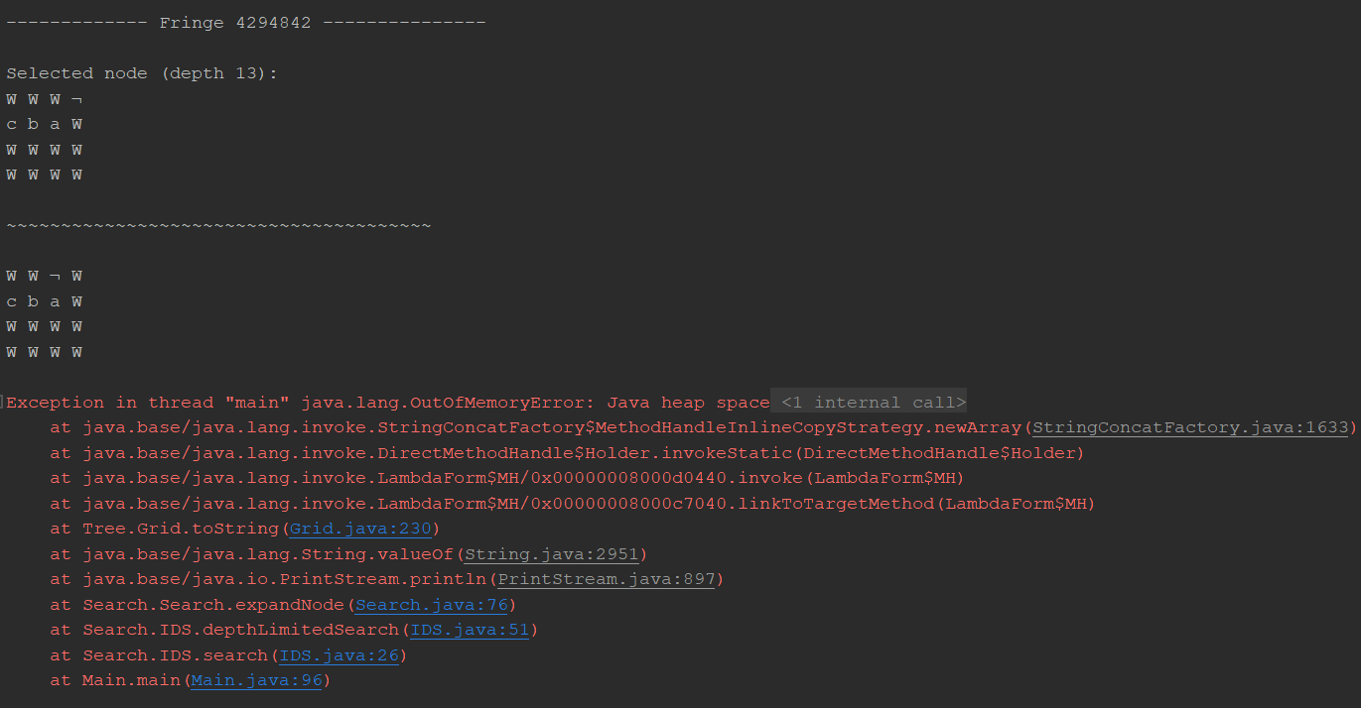
\includegraphics[height=0.43\textheight]{IDS-2-2.png}
	\end{figure}
	
	\newpage
	\subsection{A* Heuristic Search}
	\textbf{Example 1 (depth 3):}
	
	A* Search works differently to the other searches in the sense that it is an informed search, meaning the algorithm has additional information in regards to what node it should select next to expand.
	
	Looking through a simple example, we can see that a solution that has a depth of 3 can be found by expanding 3 nodes.
	
	\begin{figure}[h]
		\centering
		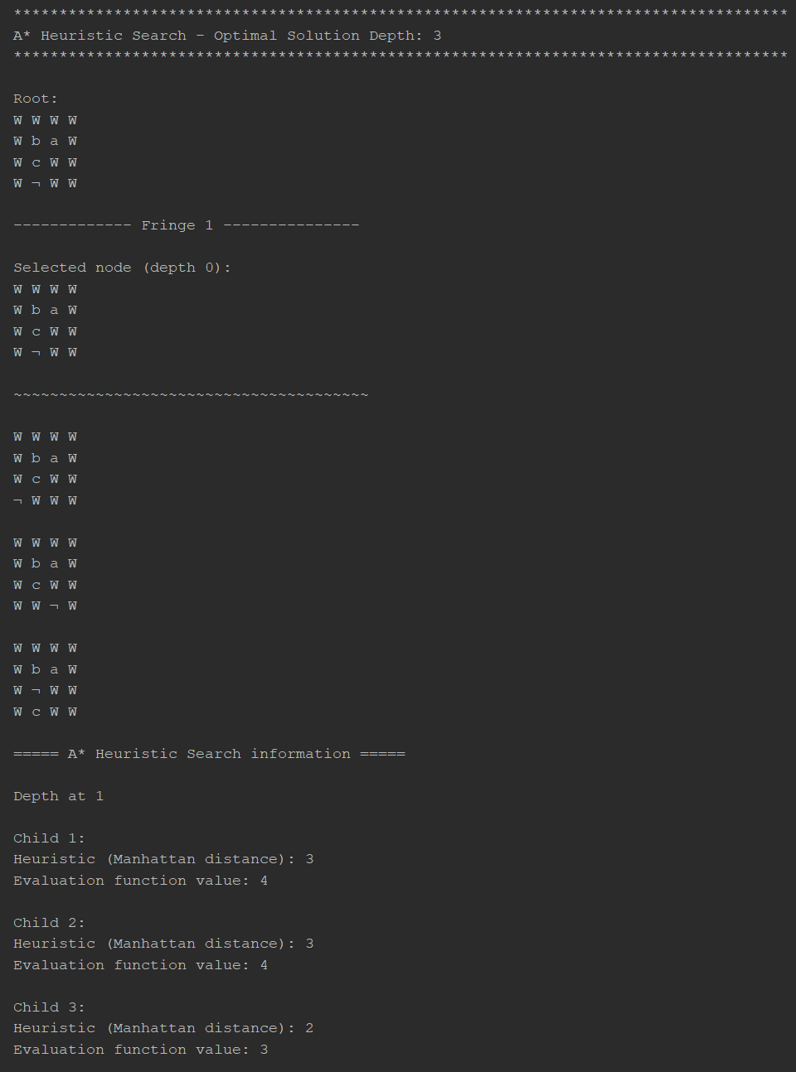
\includegraphics[height=0.75\textheight]{AStar-1-1.png}
	\end{figure}

	\newpage
	Since the third child has the lowest evaluation function value (current depth of 1 plus the heuristic of 2), the \textbf{PriorityQueue} prioritises that as the next node, and thus it is selected as the next node to be expanded.
	
	\begin{figure}[h]
		\centering
		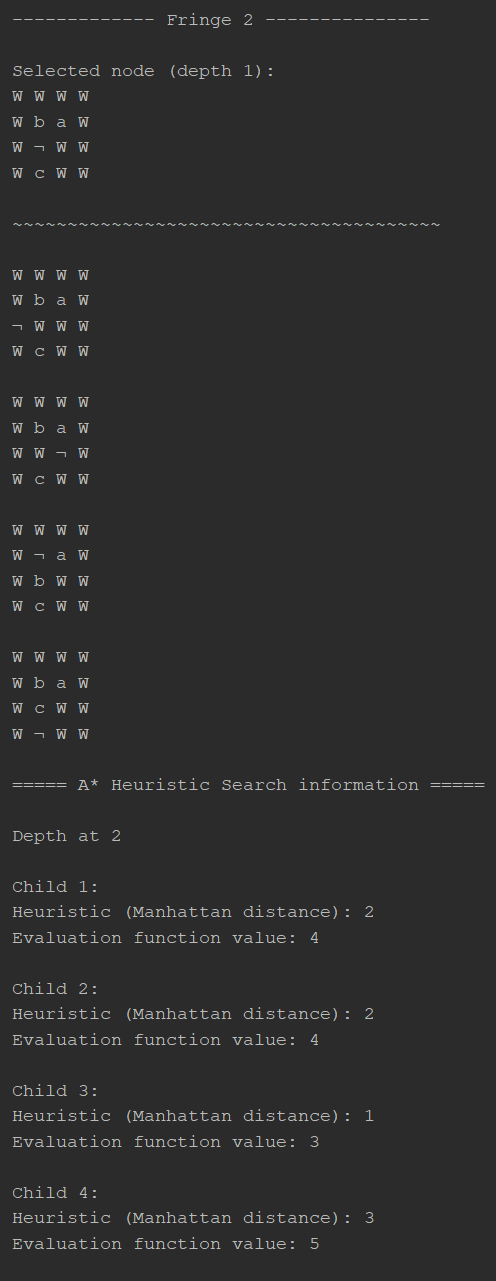
\includegraphics[height=0.75\textheight]{AStar-1-2.png}
	\end{figure}

	\newpage
	In the next step, we select the third child from the \textbf{Fringe 2} node expansion seen above. Despite the fact that it has a higher depth than some of the other possible nodes that can be expanded, its evaluation function is lower thanks to the fact that the heuristic is merely 1.
	
	\begin{figure}[h]
		\centering
		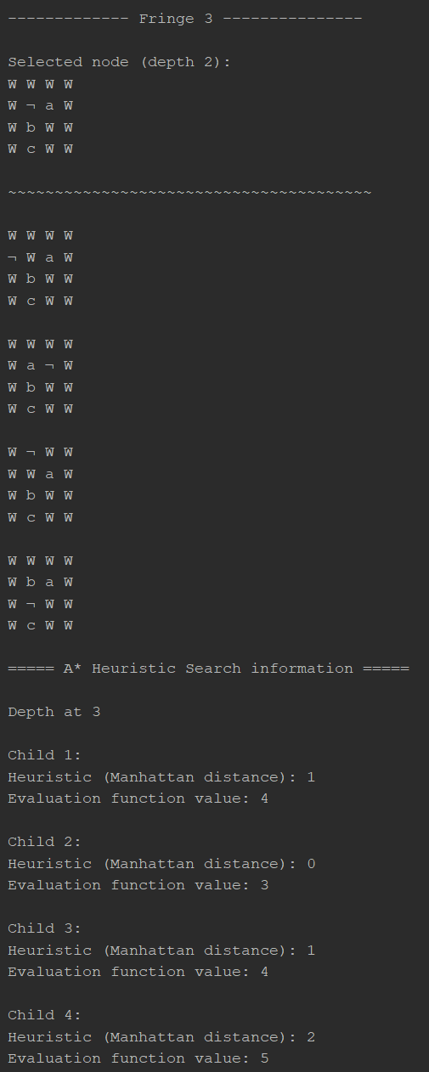
\includegraphics[height=0.75\textheight]{AStar-1-3.png}
	\end{figure}

	\newpage
	We have now found a solution, which the \textbf{PriorityQueue} will select regardless as it has the lowest evaluation function value.
	
	\begin{figure}[h]
		\centering
		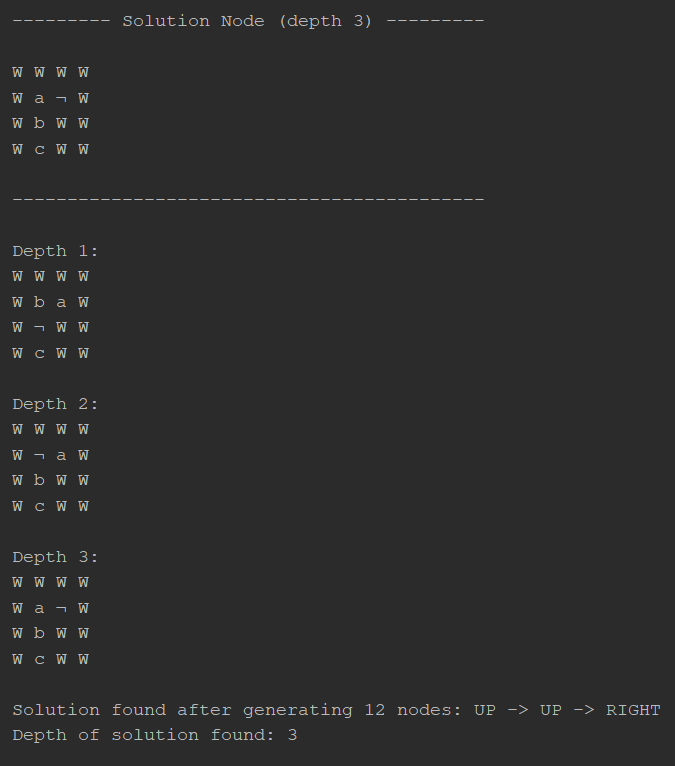
\includegraphics[height=0.75\textheight]{AStar-1-4.png}
	\end{figure}

	\newpage
	\textbf{Example 2 (depth 15):}
	
	Since A* is a smarter searching algorithm, it is capable of solving problems that the other uninformed search methods cannot due to \textbf{Java heap space errors}. For instance, it is able to find a solution for the problem that has an optimal solution at depth 15 that IDS was unable to find.
	
	\begin{figure}[h]
		\centering
		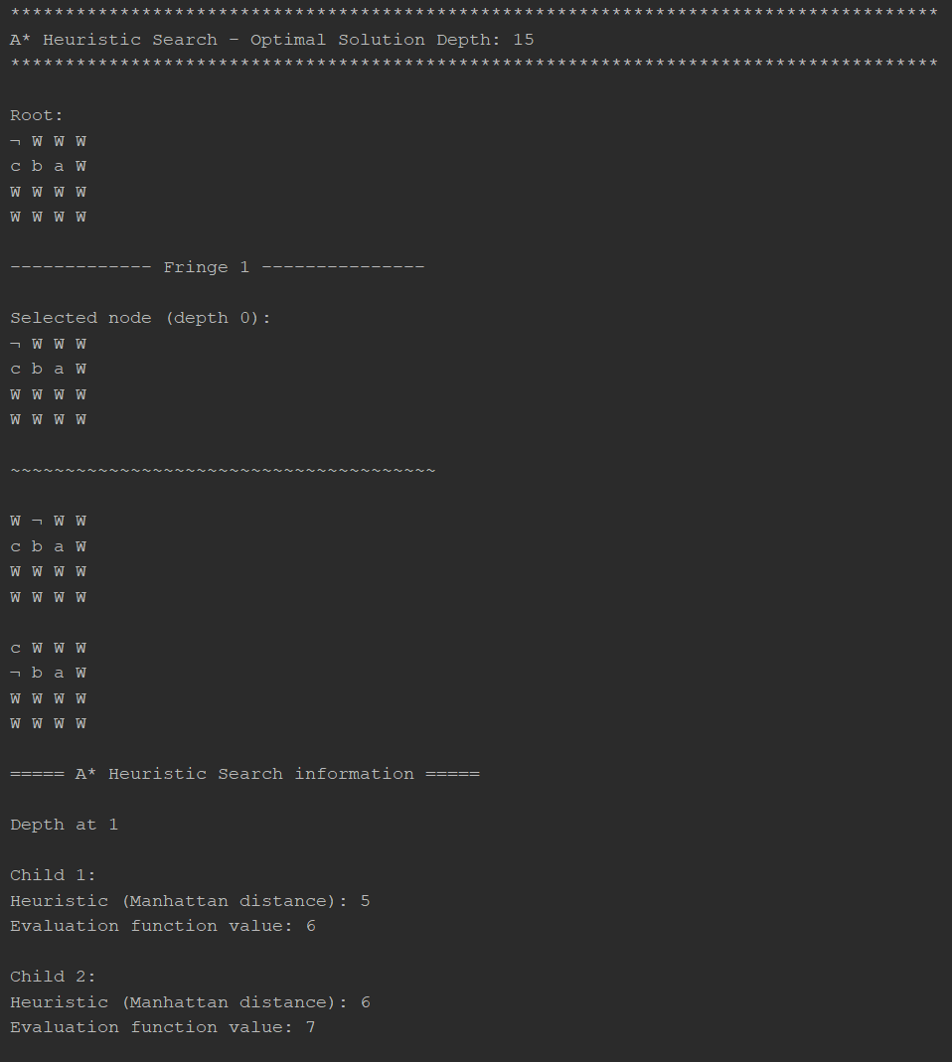
\includegraphics[height=0.75\textheight]{AStar-2-1.png}
	\end{figure}

	\newpage
	The next node that is expanded is the one with the lowest value from the evaluation function, which was the first child in this case.
	\begin{figure}[h]
		\centering
		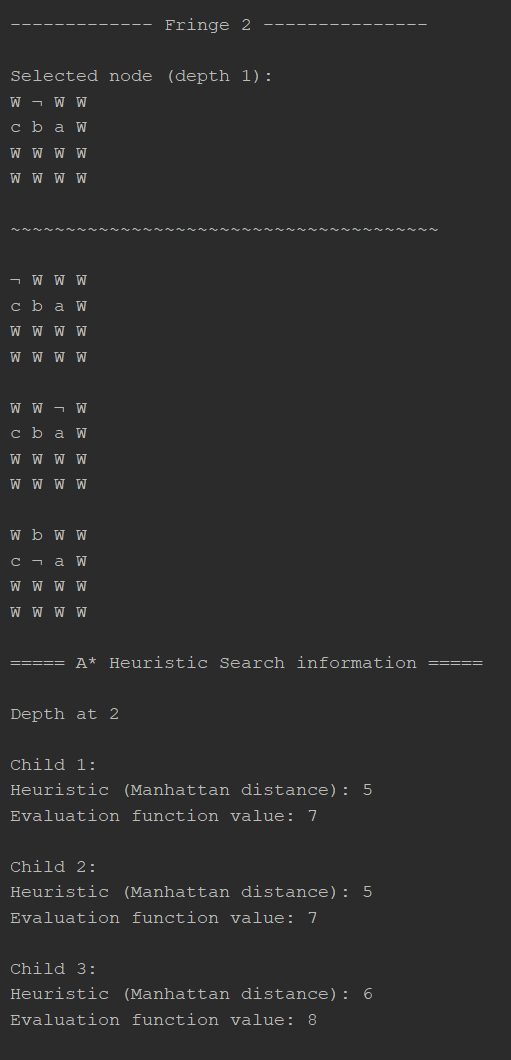
\includegraphics[height=0.75\textheight]{AStar-2-2.png}
	\end{figure}

	\newpage
	This process continues until a solution is found - here is the last node expansion performed before the goal state is discovered.
	\begin{figure}[h]
		\centering
		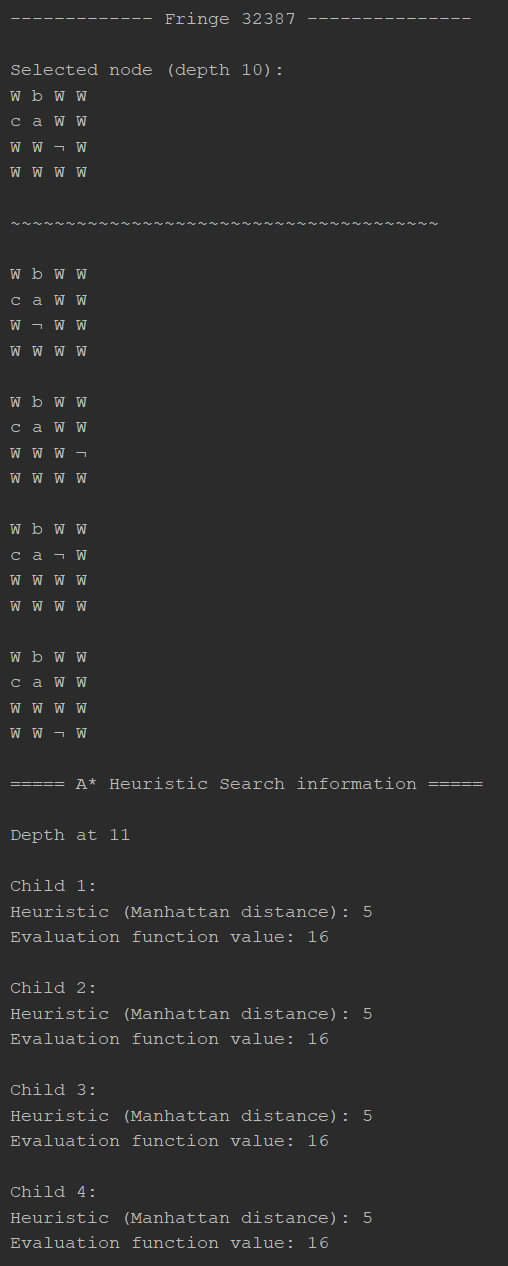
\includegraphics[height=0.75\textheight]{AStar-2-3.png}
	\end{figure}

	\newpage
	You would have noticed that the last expanded node does not contain the solution - this is because these nodes have an equal evaluation function value, so the way that they are selected in this situation is completely down to the implementation of the Java \textbf{PriorityQueue} structure. The solution node can actually be seen being generated in the node generation labelled \textbf{Fringe 32385}, two nodes before the point at which the final expansion took place.
	\begin{figure}[h]
		\centering
		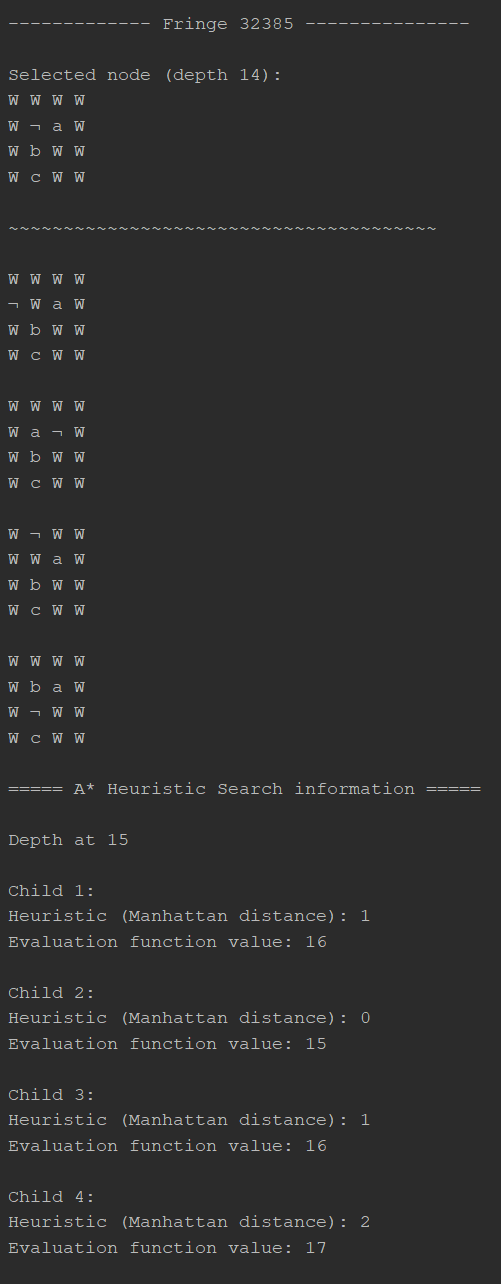
\includegraphics[height=0.75\textheight]{AStar-2-4.png}
	\end{figure}

	\newpage
	The following solution is then found, which corresponds to the optimal solution that exists at 15 steps.
	\begin{multicols}{2}[\columnsep=2cm]
		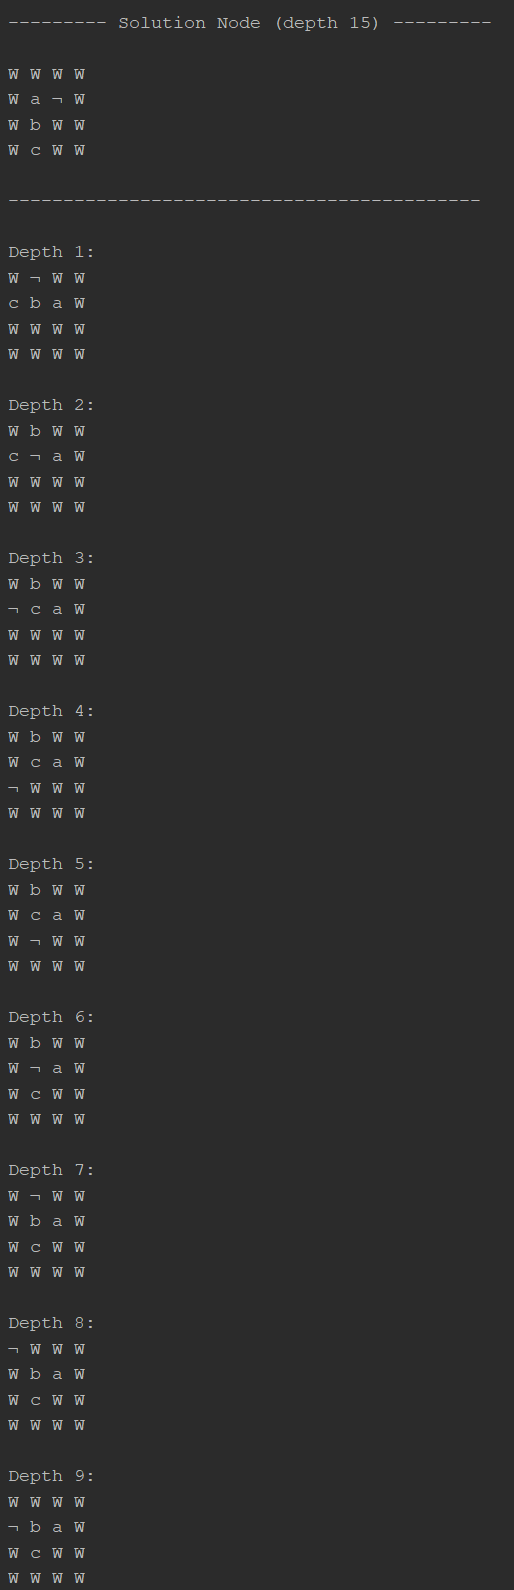
\includegraphics[height=0.8\textheight,keepaspectratio]{AStar-2-5-1.png}
		\columnbreak
		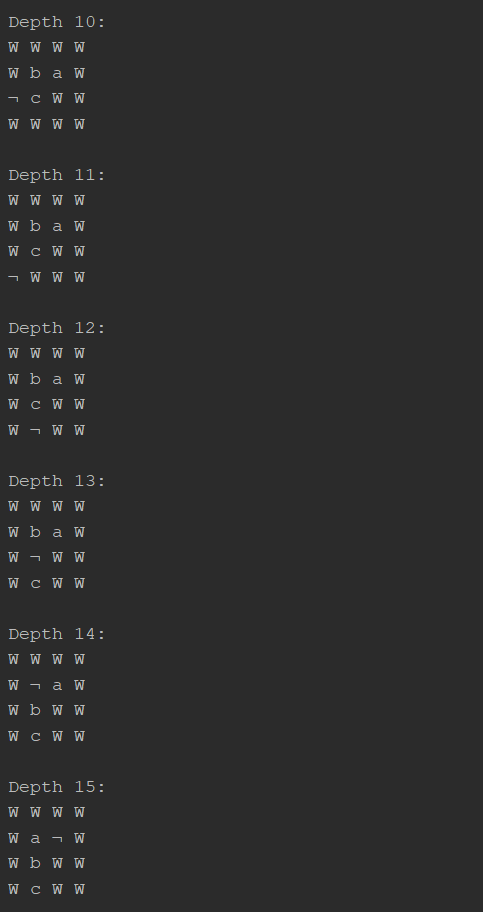
\includegraphics[height=0.8\textheight,keepaspectratio]{AStar-2-5-2.png}
	\end{multicols}

	\begin{figure}[h]
		\centering
		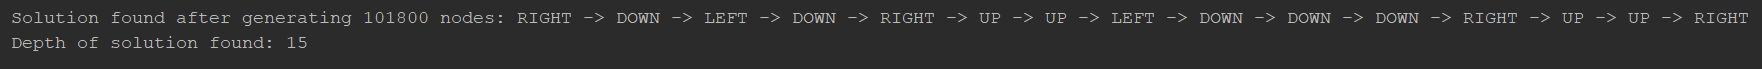
\includegraphics[width=\textwidth,keepaspectratio]{AStar-2-6.png}
	\end{figure}
	
	\newpage
	\section{Scalability Study}
	As explained above, the scalability study was conducted using 21 states, each of which corresponded to a problem that had an optimal solution from 0 to 20. For completeness, I have attached these initial states, as seen in appendix \ref{appendix:start}.
	\begin{figure}[h]	
		\centering
		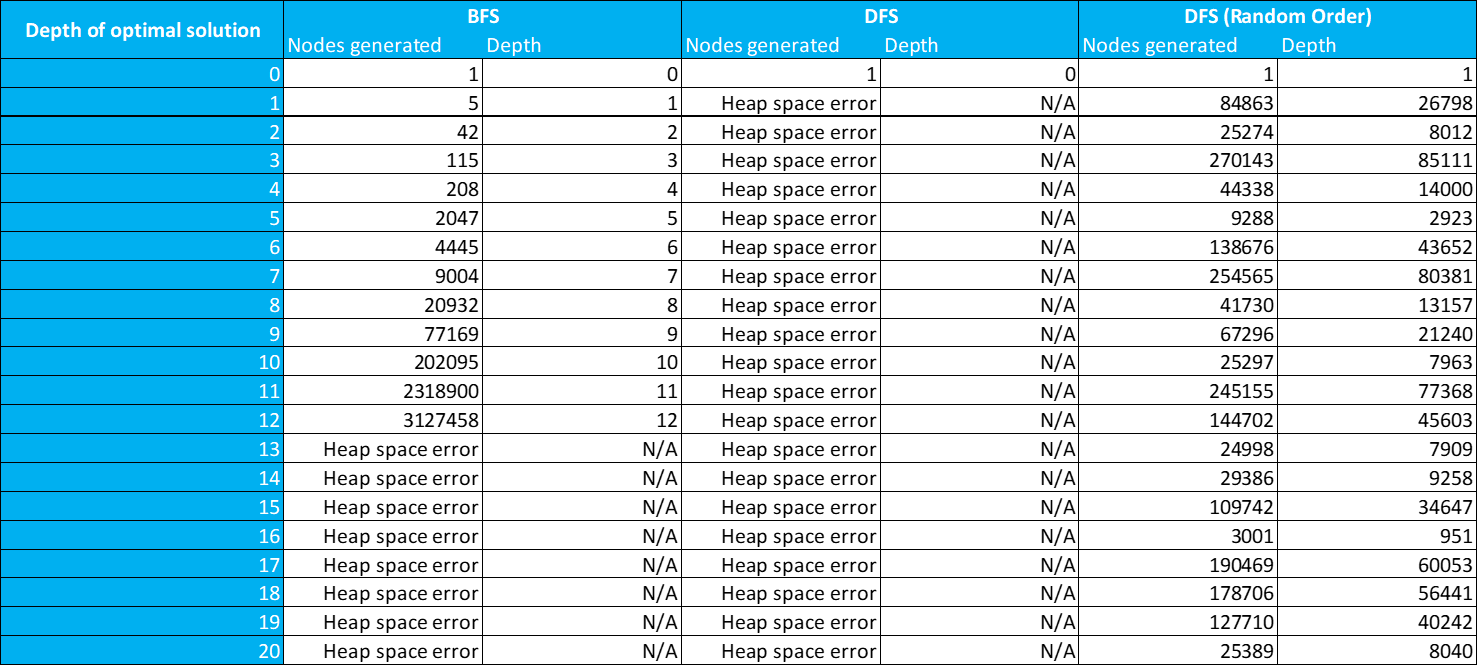
\includegraphics[width=\textwidth,keepaspectratio]{Results-1.png}
	\end{figure}
	\begin{figure}[h]	
		\centering
		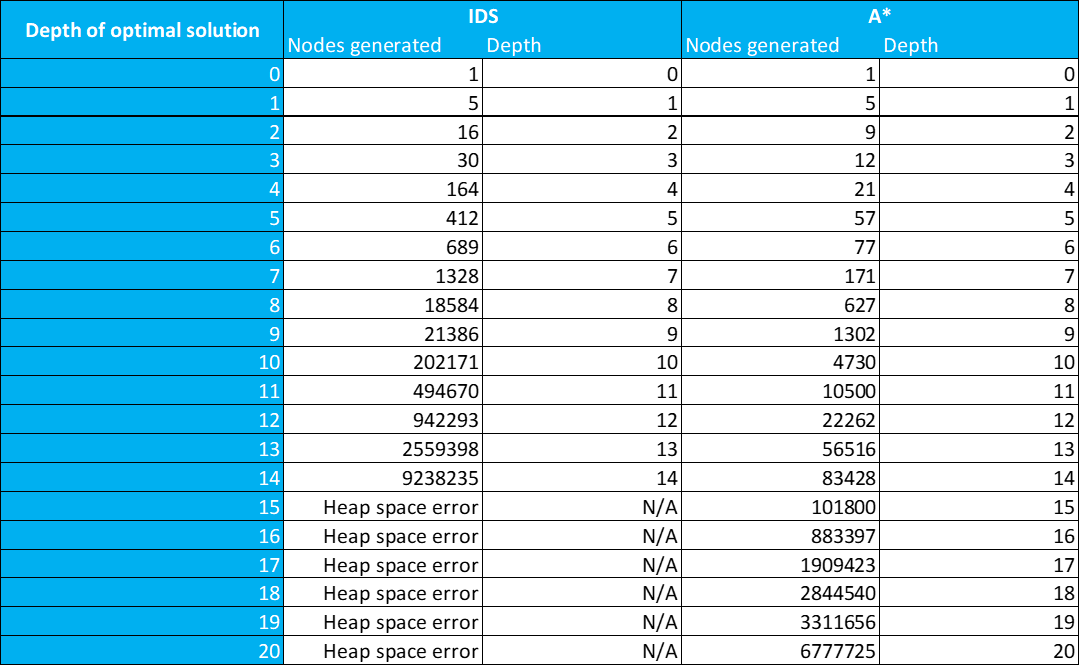
\includegraphics[width=0.75\textwidth,keepaspectratio]{Results-2.png}
	\end{figure}

	\newpage
	The below graph visualises these results. Take note of the logarithmic scale used for the nodes generated.
	\begin{figure}[h]	
		\centering
		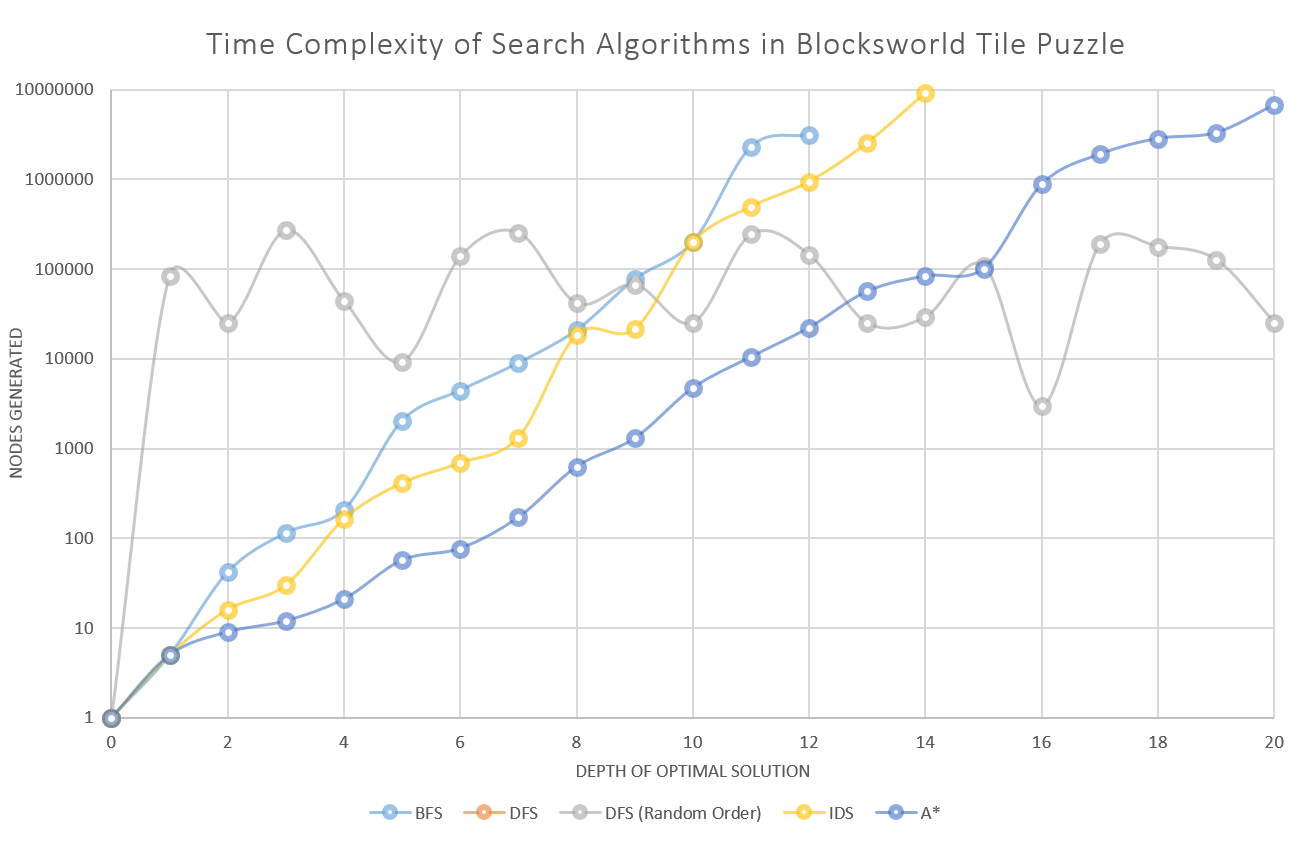
\includegraphics[height=0.5\textheight,keepaspectratio]{Results-Plot.png}
	\end{figure}

	From this data, you may extrapolate that the DFS with a random order is the best performing algorithm for problems with larger depth solutions. However, although it may be quicker to find these solutions, they are almost guaranteed to not be \textbf{optimal}. It is also worth noting that due to the arbitrary nature of this algorithm, it is actually the worst performing search at the earlier depth problems.
	
	Looking at the other algorithms, it is clear that A* is the best performing algorithm in terms of time complexity, however it is also clear that it is exponential based on the problem size. BFS and IDS would continue to rise exponentially too if they did not run into space complexity issues, but have a worse time complexity than A*. For the most part, IDS is better than BFS, but this is dependent on whereabouts in the tree structure the goal state is located.
	
	\newpage
	\section{Extras and Limitations}
	
	
	\newpage
	\begin{appendices}
		\section{Problem Start States}
		\label{appendix:start}
		
		\begin{center}
			\begin{tabular}{c c c c}
				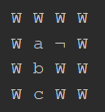
\includegraphics[width=0.135\textwidth,keepaspectratio]{State-0.png} & \includegraphics[width=0.135\textwidth,keepaspectratio]{State-1.png} & \includegraphics[width=0.135\textwidth,keepaspectratio]{State-2.png} & \includegraphics[width=0.135\textwidth,keepaspectratio]{State-3.png} \\
				State 0 & State 1 & State 2 & State 3 \\
				\includegraphics[width=0.135\textwidth,keepaspectratio]{State-4.png} & \includegraphics[width=0.135\textwidth,keepaspectratio]{State-5.png} & \includegraphics[width=0.135\textwidth,keepaspectratio]{State-6.png} & \includegraphics[width=0.135\textwidth,keepaspectratio]{State-7.png} \\
				State 4 & State 5 & State 6 & State 7 \\
				\includegraphics[width=0.135\textwidth,keepaspectratio]{State-8.png} & \includegraphics[width=0.135\textwidth,keepaspectratio]{State-9.png} & \includegraphics[width=0.135\textwidth,keepaspectratio]{State-10.png} & \includegraphics[width=0.135\textwidth,keepaspectratio]{State-11.png} \\
				State 8 & State 9 & State 10 & State 11 \\
				\includegraphics[width=0.135\textwidth,keepaspectratio]{State-12.png} & \includegraphics[width=0.135\textwidth,keepaspectratio]{State-13.png} & \includegraphics[width=0.135\textwidth,keepaspectratio]{State-14.png} & \includegraphics[width=0.135\textwidth,keepaspectratio]{State-15.png} \\
				State 12 & State 13 & State 14 & State 15 \\
				\includegraphics[width=0.135\textwidth,keepaspectratio]{State-16.png} & \includegraphics[width=0.135\textwidth,keepaspectratio]{State-17.png} & \includegraphics[width=0.135\textwidth,keepaspectratio]{State-18.png} & \includegraphics[width=0.135\textwidth,keepaspectratio]{State-19.png} \\
				State 16 & State 17 & State 18 & State 19
			\end{tabular}
		
			\begin{figure}[h]	
				\centering
				\includegraphics[width=0.135\textwidth,keepaspectratio]{State-20.png}
			\end{figure} 
			State 20
		\end{center}
	
		\section{Code}
		\label{appendix:code}
		
	\end{appendices}
	
\end{document}